\documentclass[11pt]{exam}
\usepackage[margin=1in]{geometry}
\usepackage{amsmath,amsfonts,amssymb,amsthm,enumerate}
\usepackage{multicol}
\usepackage[]{graphicx}
\addtolength{\footskip}{2\baselineskip} % to lower the page numbers
\title{\vspace{-0.5in} Math 115 \\ Worksheet Section 1.1}
\date{}


\theoremstyle{definition}
\newtheorem{problem}{Problem}


\begin{document}
\maketitle
\vspace{-0.75in}
\begin{questions}
 \question
  	\begin{enumerate}
	\item Which of the following objects represent functions?
	
	\hspace*{.2cm}the rule that sends every non-zero number to its square and sends 0 to 1
	
	\hspace*{.2cm}the rule that sends every number to 42
	
	\begin{multicols}{3}
	 
	
	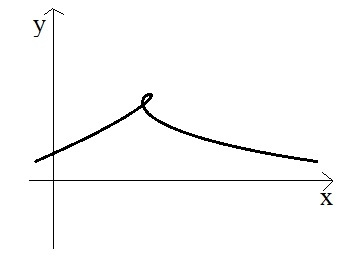
\includegraphics[width=2in]{Figures/plot1.jpg}
	
	
	
	
	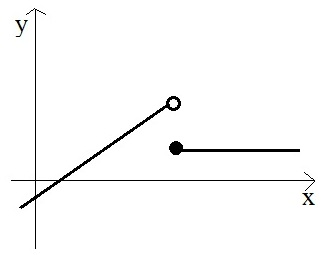
\includegraphics[width=2in]{Figures/plot2.jpg}
	
	
	
	
	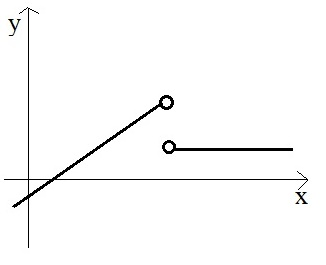
\includegraphics[width=2in]{Figures/plot3.jpg}
	
	\end{multicols}
	
	
	\begin{multicols}{4}
	
	\begin{tabular}{rl}
	$x$ & $y$\\
	\hline
	1 & 5\\
	1 & 2\\
	2 & 3\\
	3 & 4
	\end{tabular}
	
	
        \begin{tabular}{rl}
	$x$ & $y$\\
	\hline
	1 & 5\\
	2 & 3\\
	3 & 3\\
	4 & 1
	\end{tabular}
	
	 $y = x^2$
	
	 $x^2 + y^2 = 1$
	
	\end{multicols}
	
      \item  So what exactly is a \textbf{function}?	
        \vspace{0.3in}
      \end{enumerate}
\question Which graph best matches each of the following stories? Write a story for the remaining graph.
	
	\begin{enumerate}[(a)]
	\item I had just left home when I realized I had forgotten my books, so I went back to pick them up.
	\item Things went fine until I had a flat tire.
	\item I started out calmly but sped up when I realized I was going to be late.
	\end{enumerate}
	
	\begin{enumerate}[(I)]
	\begin{minipage}{.25\textwidth}
		\item 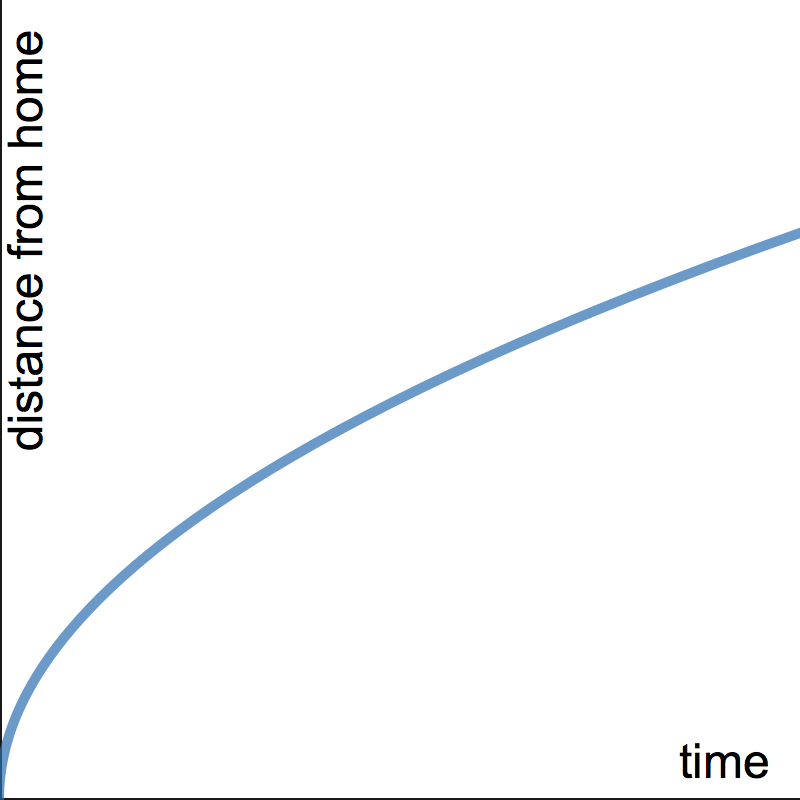
\includegraphics[scale=0.1]{Figures/graph1.png}
	\end{minipage}
	\begin{minipage}{.25\textwidth}
		\item 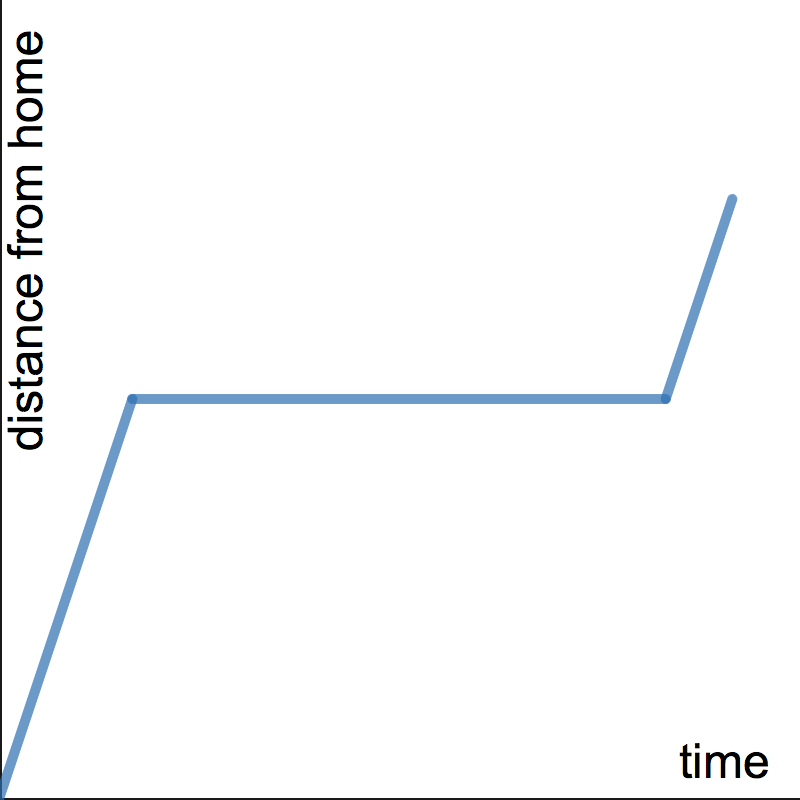
\includegraphics[scale=0.1]{Figures/graph2.png}
	\end{minipage}
	\begin{minipage}{.25\textwidth}
	\item 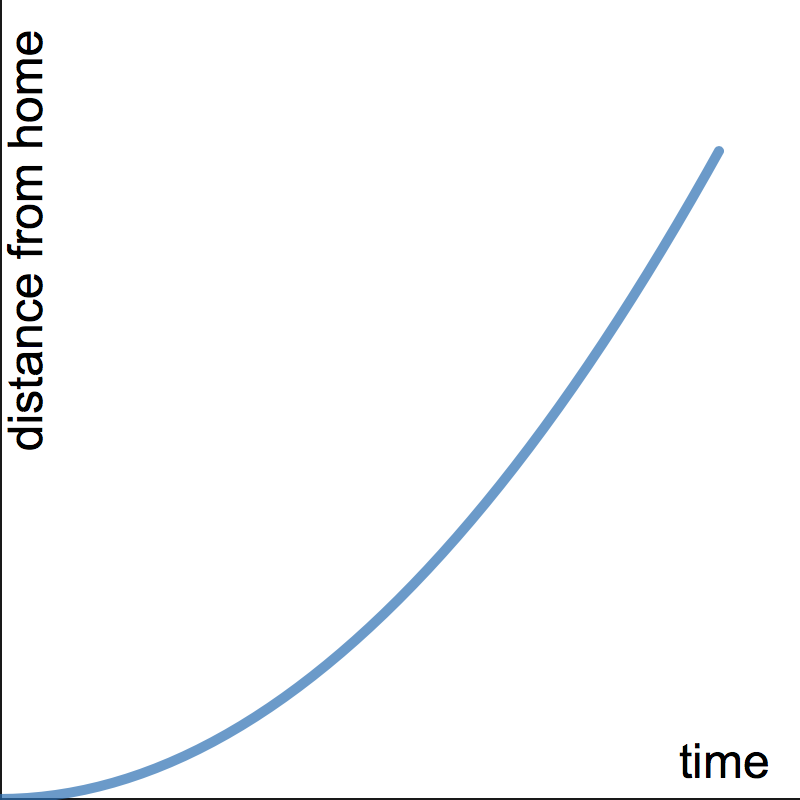
\includegraphics[scale=0.1]{Figures/graph3.png}
	\end{minipage}
	\begin{minipage}{.25\textwidth}
	\item 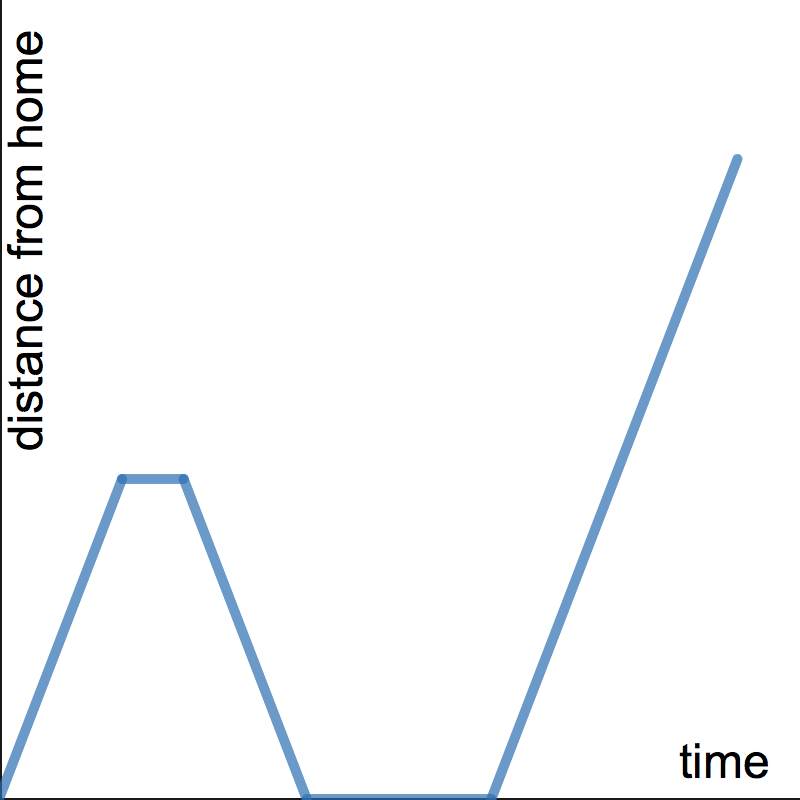
\includegraphics[scale=0.1]{Figures/graph4.png}
	\end{minipage}
	\end{enumerate}

\vskip 10mm
\pagebreak
\question
	Residents in the town of Maple Grove who are connected to the municipal water supply are billed a fixed amount monthly plus a charge for each cubic foot of water used. A household using 1000 cubic feet was billed \$40, while one using 1600 cubic feet was billed \$55.
\begin{enumerate}[(a)]
\item  What is the charge per cubic foot?
\item Write an equation for the total cost of a resident's water as a function of cubit feet of water used.
  \vspace{1in}
\item How many cubic feet of water would lead to a bill of \$100?
\end{enumerate}
\vspace{-0.5in}
\vspace{1.5in}
\question
	Match the graphs in the figure with the following equations. (Note that the \(x\) and \(y\) scales may be unequal.)
\vskip 5mm
\begin{enumerate}[(a)]
\begin{minipage}{.5\textwidth}
	\item $y=-2.27x$
	\item $y = 20.01+1.01x$
	\item $y=27.9-0.1x$
\end{minipage}
\begin{minipage}{0.5\textwidth}
	\item $y=0.1x-27.9$
	\item $y=-5.7-200x$
	\item $y=x/3.14$
\end{minipage}
\end{enumerate}
\vskip 5mm
\begin{enumerate}[(I)]
%cfe
	\begin{minipage}{.35\textwidth}
	\item 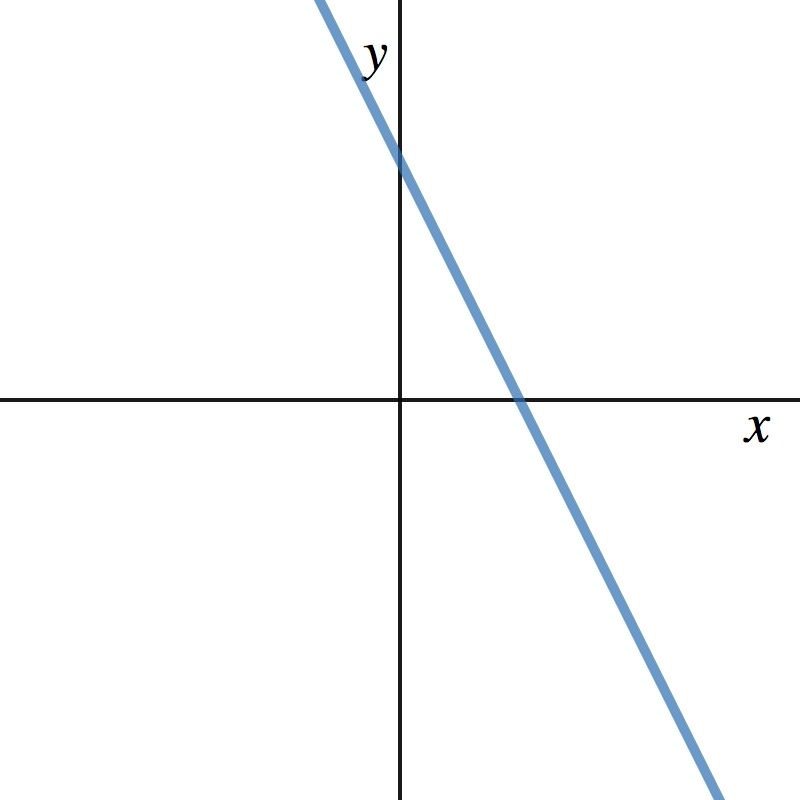
\includegraphics[scale=0.1]{Figures/linearI.png}
	\end{minipage}
	\begin{minipage}{.35\textwidth}
	\item 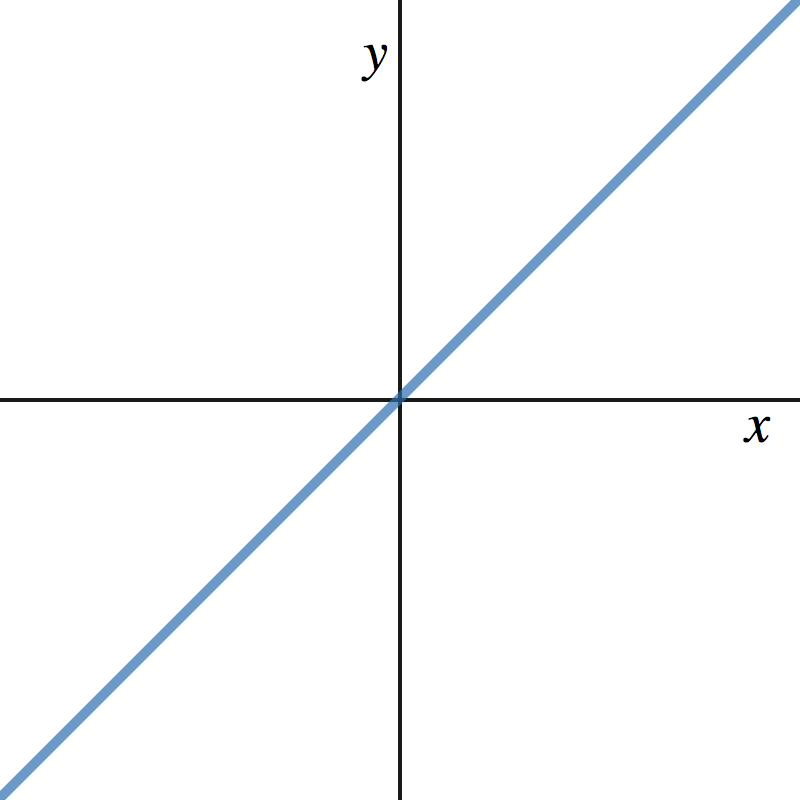
\includegraphics[scale=0.1]{Figures/linearII.png}
	\end{minipage}
	\begin{minipage}{.35\textwidth}
	\item 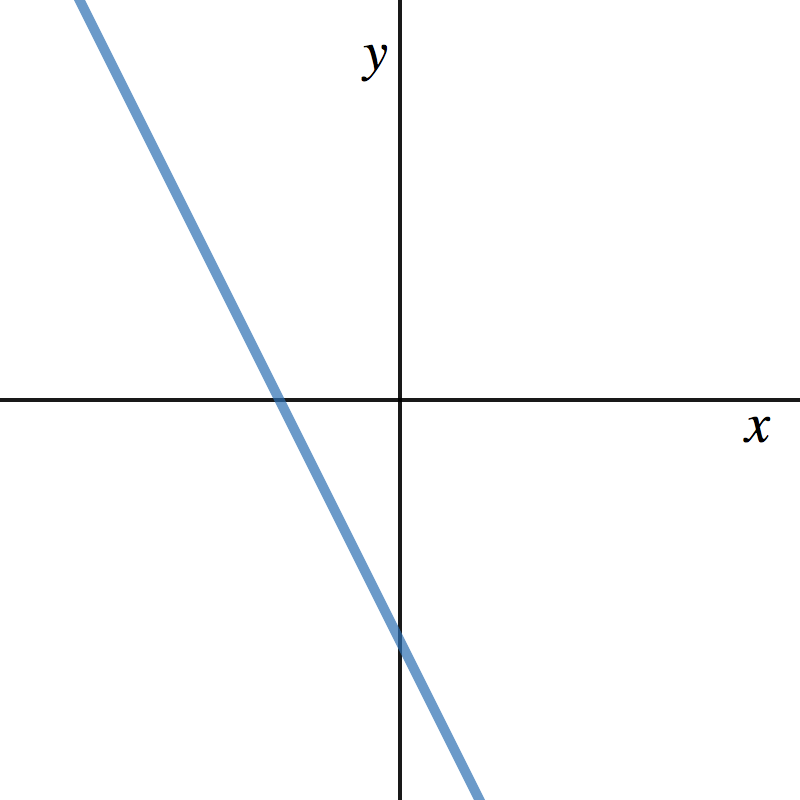
\includegraphics[scale=0.1]{Figures/linearIII.png}
	\end{minipage}
\vskip 5mm
	\begin{minipage}{.35\textwidth}
	\item 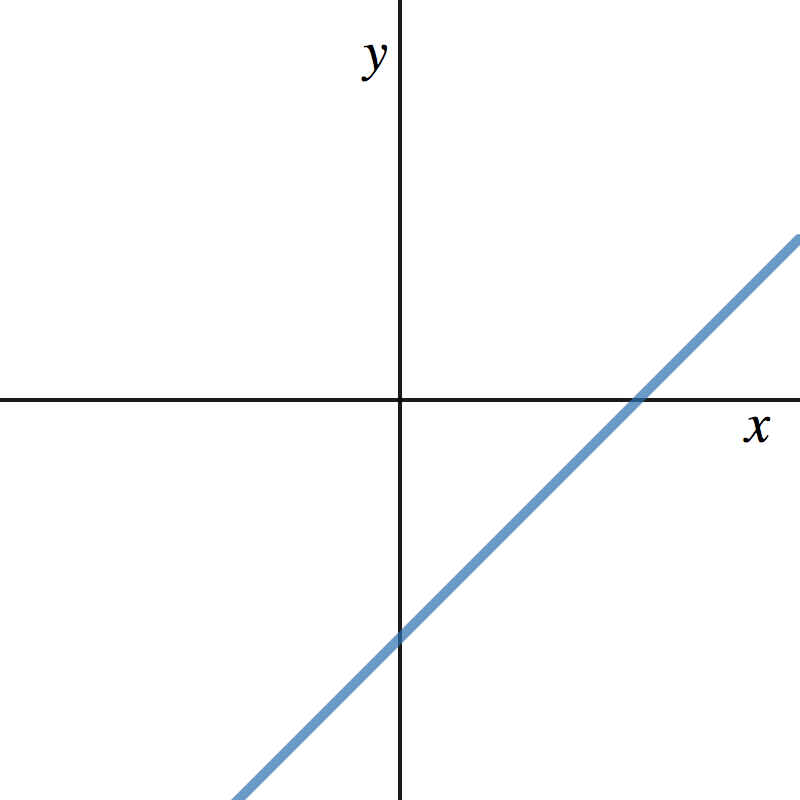
\includegraphics[scale=0.1]{Figures/linearIV.png}
	\end{minipage}
	\begin{minipage}{.35\textwidth}
	\item 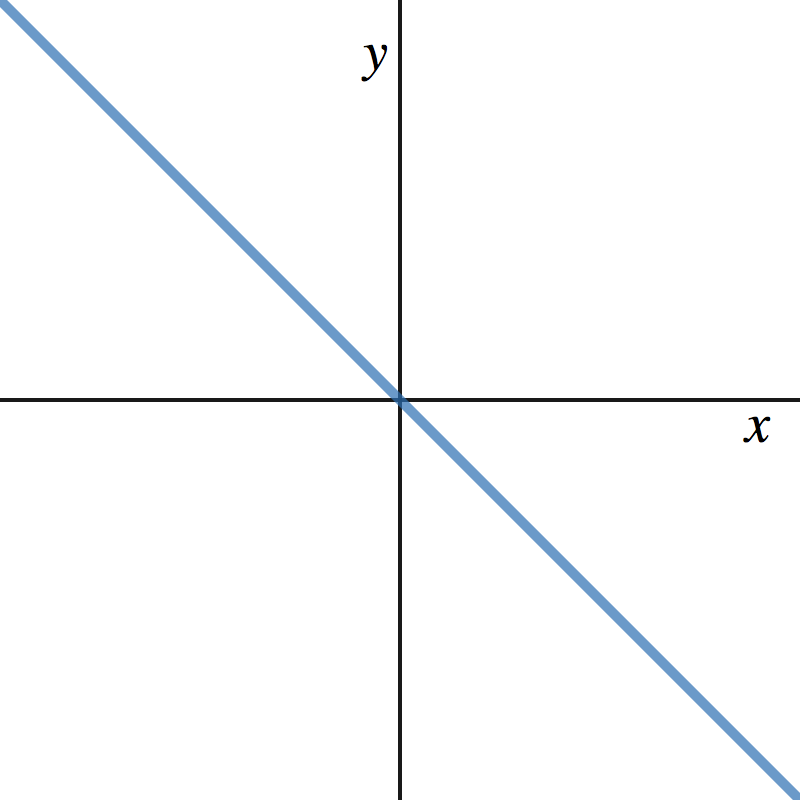
\includegraphics[scale=0.1]{Figures/linearV.png}
	\end{minipage}
	\begin{minipage}{.35\textwidth}
	\item 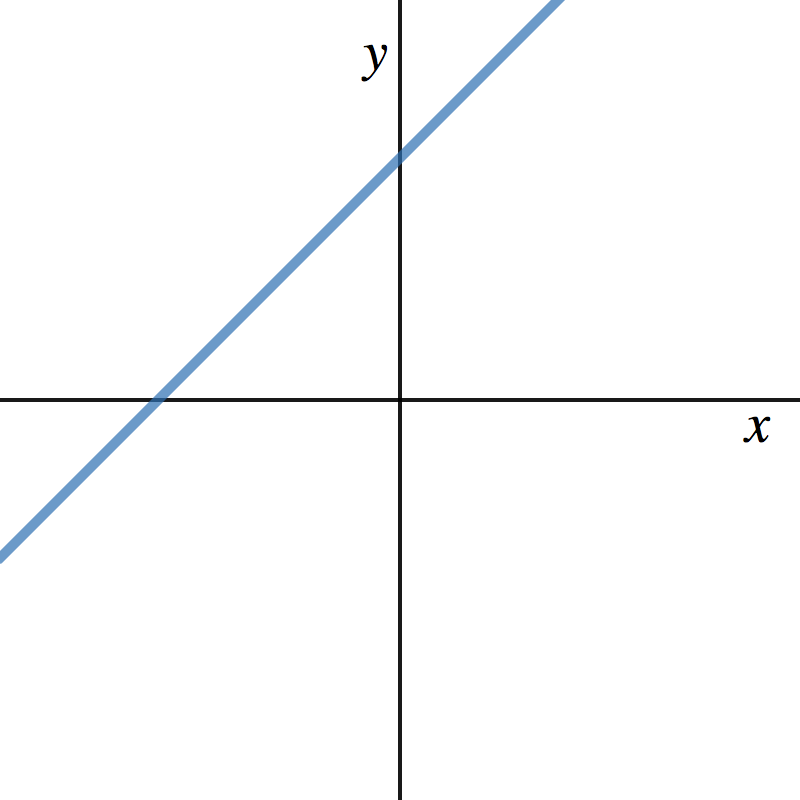
\includegraphics[scale=0.1]{Figures/linearVI.png}
	\end{minipage}
\end{enumerate}
\end{questions}
\end{document}
%%% Local Variables:
%%% mode: latex
%%% TeX-master: t
%%% End:
